%!TEX root = ../talk.tex
\chapter{Overview and Comparison of P2P File Synchronization and Storage Solutions}
\markboth{Overview and Comparison of P2P File Synchronization and Storage Solutions}{}
\chaptauthors{Josua Fr\"ohlich, Simon Ruesch}

\Kurzfassung{
This is where the abstract will go.
}

\newpage

% the table of contents
\minitoc

\newpage

\section{Introduction and Problem Statement}
Today, file synchronization and storage is demanded more than ever. The average user owns multiple devices that are continuously connected to the internet and uses the device which is the most practical for his current situation. As a consequence, users require their files to be up-to-date at all times regardless of which device the user wants to access the files on. A second aspect is that there is an ever increasing demand for systems which allow file sharing between users, such that multiple people can work on the same files independently, whether at the same time or not.

In general, the existing file synchronization and storage systems can be categorized into two groups: Client-Server based distributed file storage systems (also sometimes referred to as Cloud storage systems) and Peer-to-Peer file storage systems. Since giving a comprehensive treatment to both of those categories would be beyond the scope of this seminar thesis, the focus here lies on Peer-to-Peer file storage systems, henceforth called P2P file storage systems.

This seminar thesis aims to give an overview over the current available P2P file storage systems, to categorize them according to their different aspects and to compare their assets and drawbacks. The findings will also be compared to a popular distributed file storage system.

In chapter \ref{sec:background} we want to give a short overview  of the background of peer-to-peer systems including historical aspects, manly predecessor approaches of file storage solutions. Chapter \ref{sec:approach}

\section{Background} % @Josua
\label{sec:background}
This section gives a short basic overview over the most important topics concerning P2P systems, file storage, and the special requirements of P2P file storage systems compared to those of traditional and distributed file storage. In the a summary of the most common drawbacks of these previous but still used systems compared to peer-to-peer systems is shown.

\subsection{File Storage}
According to The Free Dictionary\cite{thefreedictionary} the term 'file storage' describes:
\begin{quote}
A generic term for warehousing electronic files. It may refer to local storage in a PC or tablet or remote storage on the Internet. The primary storage devices are hard drives and solid state drives.
\end{quote}

Traditional or \textit{Client-Server file storage}, also called \textbf{1st generation DFS} (Distributed File System) are systems where the cloud is one (or multiple) huge file server storing all the files of multiple clients being on the same network. The main problem in such systems is the file server itself as the \textit{single point of failure} and thus the server becomes the bottleneck.

	\begin{figure}[H]
		\begin{center}
		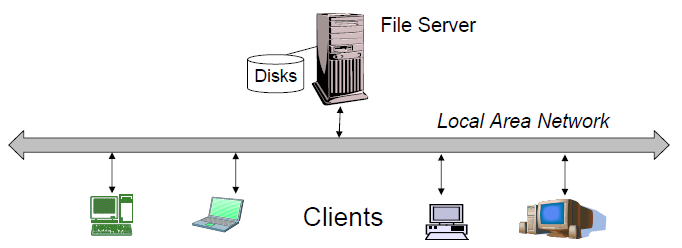
\includegraphics[scale=0.3]{Talk5/1st_gen_dfs.PNG}
		\end{center}
		\caption{1st Generation DFS \cite{wikimedia:p2p}}
		\label{1st_gen_dfs}
	\end{figure}

\textit{Distributed file systems} known as \textbf{2nd generation DFS} have some similarities to the traditional system except that files are stored to a cluster of servers, so each server stores parts of the original files. These systems are symmetric and scalable and this makes it trusted and stable.

	\begin{figure}[H]
		\begin{center}
		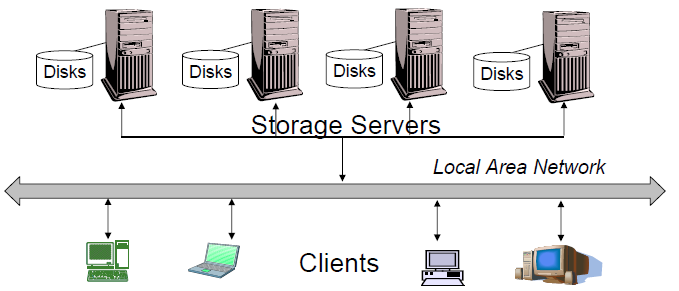
\includegraphics[scale=0.3]{Talk5/2nd_gen_dfs.PNG}
		\end{center}
		\caption{2nd Generation DFS \cite{wikimedia:p2p}}
		\label{2nd_gen_dfs}
	\end{figure}
	
The \textbf{3rd generation DFS}, namely \textit{peer to peer systems} do not have such a clear structure and separation between 'clients' and 'servers', each peer, which means each device connected to the network being able to store or access data on that network, also called node, is connected to other peers. The whole system is self-organizing, autonomous and heterogeneous. Peers can give access (read/write) to other peers to specific files and as long as these peers are connected to the network, the files are accessible.
	
	\begin{figure}[H]
		\begin{center}
		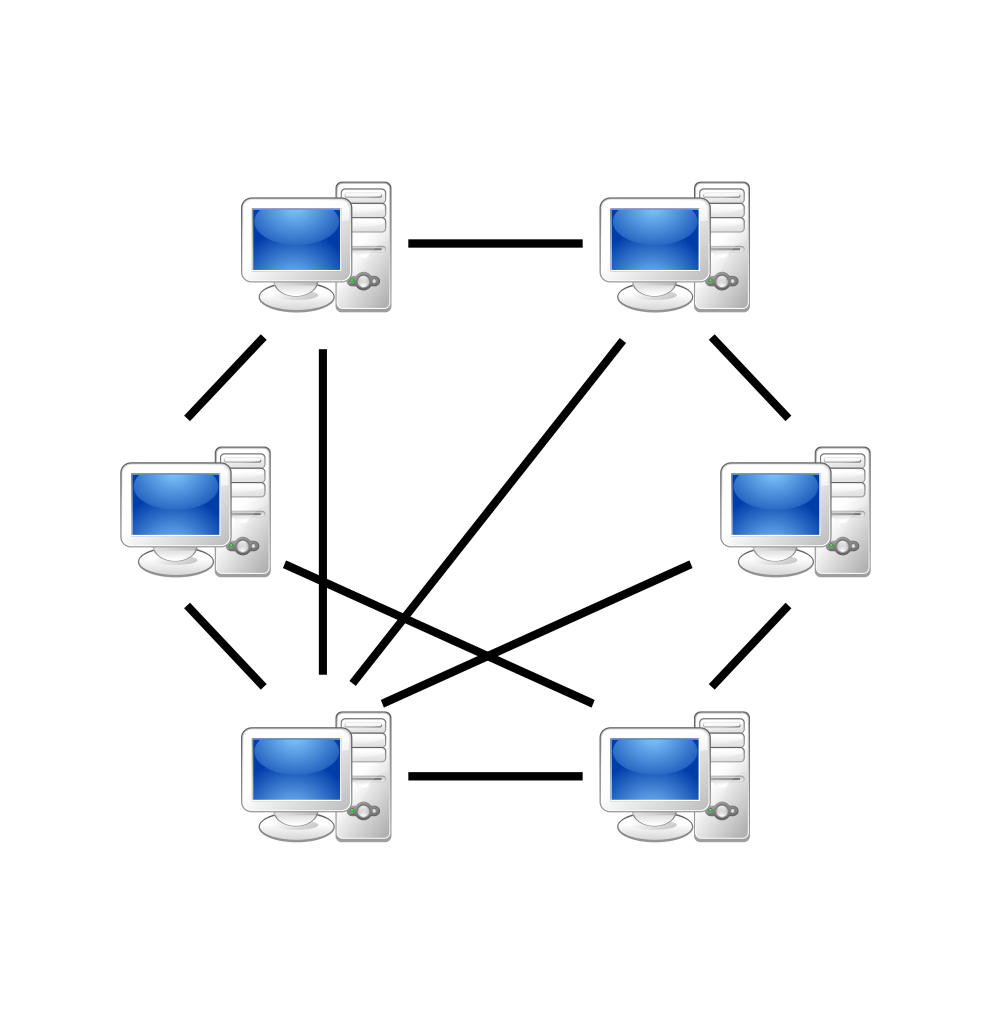
\includegraphics[scale=0.3]{Talk5/3rd_gen_dfs.PNG}
		\end{center}
		\caption{3rd Generation DFS \cite{wikimedia:p2p}}
		\label{3rd_gen_dfs}
	\end{figure}

\subsection{Peer-to-Peer}
In this section, a deeper understanding of the main ideas and goals of Peer-to-Peer systems will be given. Tough it is not possible to go very deep in this topic, the idea is to give an overview and a basis for the related work in following sections. First of all a very detailed definition of what Peer-to-Peer systems can be described as:
\begin{quote}
A distributed network architecture may be called a Peer-to-Peer (P-to-P, P2P,...) network, if the participants share a part of their own hardware resources (processing power, storage capacity, network link capacity, printers,...). These shared resources are necessary to provide the Service and content offered by the network (e.g. file sharing or shared workspaces for collaboration). They are accessible by other peers directly, without passing intermediary entities. The participants of such a network are thus resource (Service and content) providers as well as resource (Service and content) requestors (Servent-concept)\cite{ptp:definition}.
\end{quote}

Apparently the concept behind P2P systems is to move away from the traditional client-server architecture to get as far away from their withdrawals as possible. Instead of having one machine acting as a server only answering requests by clients when these clients send those requests. In P2P, the roles of the client and server are combined into one machine (hereforth called peer). Peers then can form a network of peers, i.e., a peer-to-peer network.)

Advantages and disadvantages (no single point of failure, peering may be complicated, may be difficult to prevent freeloading, security)

Maybe some pictures

Generally four different types of P2P networks are classified: (give examples)
\begin{enumerate}
	\item \textbf{Centralized P2P} which show similarities to the classical client-server model where peers in fact communicate directly with each other but with the help of a central server. (Napster, central peer serves as directory)
	\item \textbf{Hybrid P2P} provide 'super peers' to find other peers and resources. Peers communicate to these super peers until the resource is found and thus the peers can communicate directly. (Skype)
	\item \textbf{Pure P2P}, also known as \textit{unstructured P2P} systems are systems where where all peers are equally powerful communicating without any server or super peer, so peers communicate directly and act as relays to find resources. (BitTorrent)
	\item \textbf{Structured P2P} are similar to pure P2P but however the peers are organized in a specific structure, e.g. a tree to enhance peer and resource detection \cite{ptp-introduction:tomptp}. (Explain DHT)
\end{enumerate}

Peer-to-peer networks often lack of having enough peers continuously connected to the network. Where peers are defined as some volunteers helping for important files enable fast transfer speed.

\subsection{Problems of Common Sync and Sharing Services}
(Change formulation, include reference http://hive2hive.com/)Although many well-known synchronization and sharing services exist, most of them exhibit the following drawbacks:

    centralized client-server approaches, data resides in large, external data centers
    single-point-of-failure, vulnerable to targeted attacks
    often not scalable
    private data is not encrypted
    user control is revoked, no control over who has access to the private data
    user is bound to the respective pricing and terms of service
    no version control, no conflict management

\section{Approach} % @Simon
\label{sec:approach}
This section describes the criteria we chose to classify the different file storage systems. The criteria were chosen to fit what we feel are the most important aspect that a prospective user considers before making the decision of which file storage system to use. The following criteria were chosen for classification and a justification for each choice is given.

\subsection{Criteria}
\begin{itemize}
\item Peering Scheme: How are peers connected, where is user data stored, how do users communicate and what messages do they exchange?
This classification criteria describes the technical aspects of the peer-to-peer system. As described in Section 2 (include refrence) there are many different forms of peering schemes for peer-to-peer networks. It also may be important for users to know how and where their data is physically stored in the network. Some users may be weary of storing their personal data on the machine of a stranger, even if the data is divided into chunks and encrypted. This aspect also deals with how peers can share data with each other and which communication possibilities exist. 

\item Encryption: Are the communication between peers and the files stored encrypted and with which algorithm?

\item Trust and Integrity: How is trust established between peers? How are files and communication protected against fraudulent users and attacks?

\item Payment Scheme: Is the system free or paid? Who gets paid what under which circumstances?
Of course, a user is more likely to use a system the cheaper it is. However, there is also the possibility for users to earn money, e.g., by offering up their excess storage space.

\item Fairness: How is the workload distributed in the system especially considering the heterogeneous hardware used by the peers?

\item Fault-tolerance and Availability: How does the system guarantee that files are available to the users at all time?

\item Type of Distribution: Is the system only a library or a dedicated software client?
This aspect determines the ease of use of the system, but also if a expert user can build his or her own application on top of the provided system.

\item Source code availability: Is the system open-source or closed source?
This aspect is most relevant to application developers but might also be of interest for conventional users. If a system is open source, an application developers can make changes to the program code and may also contribute to future releases of the system. However, this can also be detrimental. Programmers may be able to change certain parts of their application which in turn may bypass security and fairness concepts normally applied in the system. For example, it might be possible for a malicious programmer to disable storage of data from other users while he or she stores large amounts of data of their own on other peers. In a different, more extreme example, a malicious programmer can commit changes to the public source code that contains backdoors to the encryption algorithms, allowing the programmer to access files which he or she is not normally authorized to access. The feasibility of this example depends on how many people are involved with the development of the open source project and how skilled the owners of the code are at detecting such malicious changes.
Closed source code can also be disadvantageous. If the source code is not accessible, users have to trust the developer that the security algorithms are properly implemented and that their data is only accessible to authorized parties. With open source code, an adept user can at all times verify the quality of the security scheme. Also, the more developers that are actively working on the open source project and verifying commits, the smaller is the possibility of malicious code sneaking in.

\item User base: How many users does the system currently have? Is the system intended for businesses or private users?
Firstly, the amount of users already using the system may be an indication of the quality of the system to prospective users. Also, there exists the network effect which may make it more useful for users to use a system which is already widely established instead of one which is only used by few people. Additionally, an open source system with many active users and developers may be more secure than ones with a smaller install base. However, a larger user base also makes the system a more desirable target of attack for malicious users. Secondly, the feature set of a system can also be geared more towards business applications instead of private users. It is usually more prudent to choose a system that is more suitable to the goals of the user.

\item Status: In what state is the system? Is it available for use, a scientific prototype or canceled?
\end{itemize}

\section{Comparisons}
In this section, we classify and compare four exemplary P2P file storage systems according to the classification criteria given in the preceding section. We also compare the P2P file storage to a popular distributed file storage system to find similarities and differences. At the end, we give a summary of the findings and highlight those findings in a table comparing thefile storage systems with each other.

\subsection{Storj} % @Josua
One can describe Storj (pronounced storage) as a completely decentralized and blockchain-based peer-to-peer cloud storage system with it's major concern on security and efficiency. Further it includes a peer-to-peer payment system service like Bitcoin \cite{storj:blog:what_is_storj}. Storj mainly consists of two applications, namely DriveShare (also called Driveminer)
and Metadisk. The former is uses unused harddrive space of users and the latter is a web-service used for file sharing.

% not 100% sure about that part ..
\textbf{Peering scheme:} There are no centralized servers but information of where other shards of a specific file are located is needed. So Storj uses a hybrid approach.

\textbf{Encryption:} Before encryption and distribution files are splitted into shards. These shards, a multiple of 8 or 32 Bit, are being added a deterministic salt, then uniquely encrypted and distributed over the network via a hash. A farmer does not get a whole copy (which means in this case all necessary shards of a file) but the shards are distributed to multiple farmers. For enhanced security for sensitive or important data it is also possible to combine shards, e.g. with garbage data or other client's data  \cite{storj:PDF}.

\textbf{Trust and Integrity} With the help of a pseudo-reputation system like advertisements in peer discovery to get data quality and type by tracking it or directly from the network evaluations are made to detect and qualify reputable peers. Storj uses a recommendation system for peers to improve the algorithm \cite{storj:PDF}.

The proof of storage and merkle audits, also audits through hash challenge ensure whether a farmer is able to proof he holds a specific file, or more precise; a specific shard and that the shard has not been changed or malicious modified by anything.

Storj uses different so called heartbeats to check whether a file is correctly shattered and stored. Shards are split into pieces and checked for fulfillment of the security requirements and modification detection. 

	\begin{figure}[ht]
		\begin{center}
		
\includegraphics[scale=0.8]{Talk5/storj_heartbeat.PNG}
		\end{center}
		\caption{Heartbeat shard audit \cite{storj:PDF}}
		\label{storj_heartbeat}
	\end{figure}

But what happens if a malicious farmer knows the decryption key of a specific file? He won't be able to complete the audits (heartbeats) for all shards since he isn't assigned to all of them. In addition this leads to the prove of redundancy of particular shards which means that each copy of a shard is unique \cite{storj:PDF}.

\textbf{Payment scheme:} On DriveShare users, the so called farmers, can lease their unused available hard drive space and get paid for this service in Storjcoin X (SJCX), that is based on Bitcoin. SJCX rewards, depending on the current crowdsale phase, are between 38'500 and 32480 SJCX per Bitcoin\cite{storj:crowdsale}. Users of Metadisk will pay bitcoin (BTC) for these harddrive space to be able to share their files.

\textbf{Fairness:} Storj has no central devices and through the \textit{Proof-of-Redundancy} it is guaranteed that the files are evenly distributed. Also prices can vary on the base of bandwidth speed and location of the peer and type of hardware provided \cite{storj:PDF}.

\textbf{Fault-tolerance and Availability:} To default there are thee copies of a shard all times accessible which means a shard gets copied to another node if a node goes offline. The user can request more copies in exchange of money. In this way, if a node fails an audit or is unreachable, the network replication process is initiated and thus the network is able to 'heal' itself.

To archive accordance of file location ad integrity over the whole network a block-chain like for Bitcoin according to Satoshi Nakamoto \cite{bitcoin} is used:

\begin{quotation}To use a basic analogy, it is easy to steal a cookie from a cookie jar in a secluded area, but it is hard to do so when the jar is instead located in the middle of a public square, being observed by thousands of people \cite{storj:PDF}.\end{quotation}

\textbf{Type of distribution:} As mentioned above, Storj consists of two applications; DriveShare and Metadisk.

\textbf{Source code availability:} Both applications (and even more Storj applications) are fully open-source \cite{storj:github}.

\textbf{User base:} There are no official up-to-date data, in addition the system is currently in beta-phase. The forum of Storj has over one thousand members \cite{storj:forum} and lets assume that there are currently even more storj users. In June 2014 Storj had about more than 3'000 users \cite{storj:crowdsale}.

\textbf{Status:} Storj is currently in beta phase and already available for use. There are three different test groups; A, B and C each with different conditions (rewarding system, requirements, starting date) \cite {storj:earlyaccess}

\subsection{Hive2Hive} % @Simon 
Hive2Hive (formerly known as Box2Box) is an open source peer-to-peer file sharing and synchronization library that started out as part of a course challenge task project and was further improved in a graduate student's project at the Communication Systems Group at the University of Zurich. (https://github.com/Hive2Hive/Hive2Hive/wiki/About-Us) It is built on top of the TomP2P library (an open source Distributed Hash Table (DHT) based key-value store) which was also developed at the Communication Systems Group. (http://tomp2p.net/)

\textbf{Peering Scheme}
Structured P2P based on the TomP2P DHT. Each peer has an id. Files are divided into chunks, a random id is generated for each chunk and stored in the metadata file of the file, the chunk is stored at the peer with the id closest to the hashed id of the chunk. The metadata file is also stored in the dht, but is only accessible to the creator of the file. ...

\textbf{Encryption}
AES for symmetrical, RSA for asymmetrical
The keys are stored in the user identity file stored in the dht, which is only accessible by the user which the identity belongs to.

\textbf{Trust \& Integrity}
There are two types of file access permission that can be given to other peers, read access and read/write access. Peers without any of those permissions cannot access a file. File chunks are signed with an MD5 hash to guarantee integrity. Peers have to verify the identity of the peers that they want to share files with themselves.

\textbf{Payment Scheme}
Hive2Hive is open source and is like most open source software free of charge to use.

\textbf{Fairness}
Since ids for file chunks are generated randomly, the file chunks are distributed equally between all peers in the long run. No prevention from peers storing an extraordinary amount of files

\textbf{Fault-tolerance and Availability}
File chunks are replicated 3 times but higher amounts can be configured

\textbf{Type of Distribution}
Hive2Hive itself is a library that provides that functionality of file sharing and synchronization. However, an end-user GUI application called Peerwasp (http://www.peerwasp.com/) is currently in development that uses Hive2Hive as a basis.

\textbf{Source code availability}
The source code of Hive2Hive, TomP2P as well as Peerwasp is freely available on Github. (https://github.com/Hive2Hive/Hive2Hive) (https://github.com/tomp2p/TomP2P) (https://github.com/PeerWasp/PeerWasp)

\textbf{User base}
No idea

\textbf{Status}
Mature library with active development

\subsection{BitTorrent Sync} % @Simon

\textbf{Peering Scheme}
There is not really a network. Files cannot be stored per se, only synchronized between multiple devices. But sharing is also possible. One device which contains the file must be online for synchronization to happen.

\textbf{Encryption}

\textbf{Trust \& Integrity}

\textbf{Payment Scheme}

\textbf{Fairness}

\textbf{Fault-tolerance and Availability}

\textbf{Type of Distribution}

\textbf{Source code availability}
BitTorrent Sync is currently closed source.

\textbf{User base}

\textbf{Status}

\subsection{AeroFS} % @Josua
AeroFS is a dedicated software client from Air Computing providing basic peer to peer solutions but some advanced functionality concerning advanced security and encryption, error and data loss prevention and everything for low costs \cite{aerofs}.

\textbf{Peering scheme:} There are basically two different peering schemes, one without Air servers, where data can be exchanged within the local area network for enhanced up-link time in comparison to internet up-links \cite{aerofs:peering_scheme} and a centralized solution with the AeroFS Team Server to back up files on a central location \cite{aerofs:peering_scheme_2}. Thus Air Computing uses a hybrid solution as a peering scheme.

\textbf{Encryption:} An end-to-end encryption solution is provided, files are encrypted before transaction using AES-256 with 2048-bit RSA and only the recipient is able to decrypt the data transfer \cite{aerofs:security}. On the servers of AeroFS are only usernames, the hashes of the passwords and the names of the access authorized users from folders stored \cite{aerofs:security_2}.

\textbf{Trust and Integrity} The amount of users from a borrower is of fixed size (but can grow), also using the AeroFS Applicance as root certificate, no other footprint will be accepted by the clients \cite{aerofs:security}.

\textbf{Payment scheme:} The basic pricing plan (Team) is free up to a user-base size of 30 \cite{aerofs:blog:30_users_free} and the business plan starts above 31 users and according to the size of the user-base the billing is done; e.g. for 40 users and the cost totals in \$600, the biggest available size on the website is 1000 users for \$15'000 per month \cite{aerofs:pricing}.

\textbf{Fairness:} Three different cloud options:
\begin{enumerate}
\item \textbf{Private Cloud}: Provides private Web Administration, manage registration and authentication of users and private Certificate Authority (CA) to manage the AeroFS public key infrastructure (PKI) for client applications
\item \textbf{Hybrid Cloud}: Supply a centrally managed file sharing platform for the employees and registration, authentication and user management is done outside the network by AeroFS.
\item \textbf{Team Server} (optional Addon): Light weight client to enable backup of files and 24/7 availability \cite{aerofs:cloud_types}.
\end{enumerate}
If a hard-drive gets too full, the versioning systems keeps track of the oldest copies and deletes them if the user runs out of space \cite{aerofs:USTO.RE}.
%%https://www.aerofs.com/developers/ --> load balancer

\textbf{Fault-tolerance and Availability:} 
% research needed

\textbf{Type of distribution:} AeroFS serves a software client for users and a admin dash panel for enhanced manageability.

\textbf{Source code availability:} AeroFS is currently closed source.
There are three different types of storage for the AeroFS Team Server:
\begin{enumerate}
\item \textbf{Linked Storage}: creates a read/write copy of organization's files on the team server. Files will be browseable.
\item \textbf{Block Storage}: compresses and de-duplicates files for enlarged disk space. Files won't be browseable.
\item \textbf{S3 Storage}: Data shared by users of an organization is stored and backed up on Amazon servers compressed and de-duplicated. Files won't be browseable \cite{aerofs:storage_types}.
\end{enumerate}

\textbf{User base:} According to the webpage \cite{aerofs} there are currently \textbf{50'000+} users.

\textbf{Status:} Available for use and costs-free.

\subsection{Dropbox}

\textbf{Peering Scheme}
Data is stored in the Amazon S3 cloud.
\textbf{Encryption}

\textbf{Trust \& Integrity}
Data is encrypted but keys are stored on dropbox servers, not on client machines

\textbf{Payment Scheme}
Freemium, base use is free, for more storage, a paid subscription is available.

\textbf{Fairness}
not applicable
\textbf{Fault-tolerance and Availability}
bö

\textbf{Type of Distribution}
Available through their website but GUI application also exists.

\textbf{Source code availability}
Closed source

\textbf{User base}
% userbase: http://thenextweb.com/insider/2014/05/29/dropbox-reaches-300m-users-adding-100m-users-just-six-months/

\textbf{Status}

\section{Summary and Conclusions} In this section, we provide a summary about the topics mentioned above and draw conclusions about the current state of the available P2P file storage systems and what the future could hold for P2P file storage.

\begin{thebibliography}{99}
	\bibitem {aerofs}
		\emph{AeroFS}
		\url{https://www.aerofs.com/},
		March, 2015.

	\bibitem {bitcoin}
		S. Nakamoto:
		\emph{Bitcoin: A Peer-to-Peer Electronic Cash System;}
		\url{https://bitcoin.org/bitcoin.pdf},
		October, 2008.

	\bibitem {bittorrentsync-2}
		J. Farina, M. Scanlon, M. Kechadi:
		\emph{BitTorrent Sync: First Impressions and Digital Forensic Implications;}
		Proceedings of the First Annual DFRWS Europe,
		\url{http://ac.els-cdn.com/S1742287614000152/1-s2.0-S1742287614000152-main.pdf?_tid=10ddb6e2-ce69-11e4-9019-00000aacb35d&acdnat=1426791318_6677afbe19d521d323605261c1d19809},
		Volume 11, Supplement 1, Pages S77\textendash S86, Volume 11, May, 2014.

	\bibitem {box2box}
		A. Lareida, T. Bocek, S. Golaszewski, C. L\"uthold, M. Weber:
		\emph{Box2Box - A P2P-based File-Sharing and Synchronization Application;}
		\url{http://www.csg.uzh.ch/csg/live/teaching/FS13/p2p/challenge/P2P2013DP_017.pdf},
		September, 2013.

	\bibitem {hive2hive}
		\emph{Hive2Hive: Open-Source Library for P2P-based File Synchronization and Sharing;}
		\url{http://hive2hive.com/},
		March, 2015.

	\bibitem {metadisk}
		S. Wilkinson, J. Lowry:
		\emph{Metadisk: Blockchain-based decentralized file storage application;}
		\url{http://metadisk.org/metadisk.pdf},
		December, 2014.

	\bibitem {p2pfswu}
		C. Wu:
		\emph{Peer-to-Peer Networks;}
		\url{http://www.csie.nuk.edu.tw/~wuch/course/csf641/csf641-04-storage.pdf},
		March, 2015.

	\bibitem {p2pfskangasharju}
		J. Kangasharju:
		\emph{Peer-to-Peer Networks Chapter 4: Peer-to-Peer Storage;}
		\url{http://www.cs.helsinki.fi/u/jakangas/Teaching/P2P/P2P-04-Storage.pdf},
		March, 2015.

	\bibitem {storj:PDF}
		S. Wilkinson:
		\emph{Storj A Peer-to-Peer Cloud Storage Network;}
		\url{http://storj.io/storj.pdf/},
		December, 2014.

	\bibitem {bittorrentsync}
		\emph{Sync;}
		\url{https://www.getsync.com/},
		March, 2015.
		
	\bibitem {storj:blog:what_is_storj}
		\emph{What ist Storj?;}
		\url{http://blog.storj.io/post/87251450053/what-is-storj},
		March, 2015.
		
	\bibitem {storj:deck}
		\emph{Storj - The Crowdsale;}
		\url{http://storj.io/crowdsale.html},
		March, 2015.
		
	\bibitem {storj:crowdsale}
		\emph{Storj Deck - Decentralized Cloud;}
		\url{http://storj.io/Deck.pdf},
		April, 2015.

	\bibitem {storj:github}
		\emph{Storj Labs;}
		\url{https://github.com/Storj/},
		March, 2015.
		
	\bibitem {ptp-introduction:tomptp}
		\emph{TomP2P: A P2P-based high performance key-value pair storage library;}
		\url{http://tomp2p.net/doc/p2p/},
		April, 2015.
		
	\bibitem {storj:forum}
		\emph{Storjtalk;}
		\url{https://storjtalk.org/},
		April, 2015.
		
	\bibitem {storj:earlyaccess}
		\emph{Storj - Early Access;}
		\url{http://storj.io/earlyaccess.html},
		April, 2015.
		
	\bibitem {aerofs:blog:30_users_free}
		Y. Sagalov:
		\emph{AeroFS is now free up to 30 users;}
		\url{https://www.aerofs.com/blog/aerofs-is-now-free-up-to-30-users/},
		April, 2015.
		
	\bibitem {aerofs:pricing}
		\emph{Pricing, AeroFS;}
		\url{https://www.aerofs.com/pricing/},
		April, 2015.
		
	\bibitem {aerofs:peering_scheme}
		\emph{Security Share and Transfer Large Files, Enterprise Solution, Aerofs;}
		\url{https://www.aerofs.com/solutions/transfer-large-files/},
		April, 2015.
		
	\bibitem {aerofs:peering_scheme_2}
		\emph{Flexible Storage for the Enterprise;}
		\url{https://www.aerofs.com/features/flexible-storage/},
		April, 2015.
		
	\bibitem {aerofs:security}
		\emph{Security, AeroFS;}
		\url{https://www.aerofs.com/security/},
		April, 2015.
		
	\bibitem {aerofs:security_2}
		\emph{AeroFS: Das bessere Dropbox? - Golem.de;}
		\url{http://www.golem.de/news/aerofs-das-bessere-dropbox-1304-98485.html},
		April, 2015.
		
	\bibitem {aerofs:storage_types}
		\emph{What Storage Types Can I Use With The AeroFS Team Server? - AeroFS Support;}
		\url{https://support.aerofs.com/hc/en-us/articles/203434524},
		April, 2015.
		
	\bibitem {aerofs:cloud_types}
		\emph{Enterprise Solution - Deployment Options, AeroFS;}
		\url{https://www.aerofs.com/features/deployment-options/},
		April, 2015.
		
	\bibitem {aerofs:USTO.RE}
		Dur\~ao et al:
		\emph{USTO.RE: A Private Cloud Storage Software System;}
		\url{http://www.researchgate.net/profile/Vinicius_Garcia/publication/262284124_USTO.RE_a_private_cloud_storage_software_system/links/5457a3f30cf2cf51648219ed.pdf},
		April, 2015.
		
	\bibitem {wikimedia:p2p}
		\emph{Peer-to-peer;}
		\url{http://en.wikipedia.org/wiki/Peer_to_peer},
		April, 2015.
		
	\bibitem {thefreedictionary}
		\emph{File Storage Definition;}
		\url{http://encyclopedia2.thefreedictionary.com/file+storage},
		April, 2015.
		
	\bibitem {ptp:definition}
		R. Schollmeier:
		\emph{A Definition of Peer-to-Peer Networking for the Classification of Peer-to- Peer Architectures and Applications;}
		\url{http://ieeexplore.ieee.org/xpls/abs_all.jsp?arnumber=990434&tag=1},
		April, 2015.

\end{thebibliography}